
\section{Seasonal and Spatial Variation}

\subsection{Springs changing concentration with season, indicating monsoonal precipitation influence}
\textcolor{red}{Systematic undulation september to october to november to april. Small amount compared to rainfall Si...} Several springs show evidence for a concentration decrease during the monsoon, as increased water flux dilutes the normal element load in the water. This is also visible in a spring time series over several months. Both sample sets display a decrease in concentration in September, where the effect of the monsoon is the greatest. It would be worth it to compare to previous literature values.??




\begin{figure}[h]
    \centering
    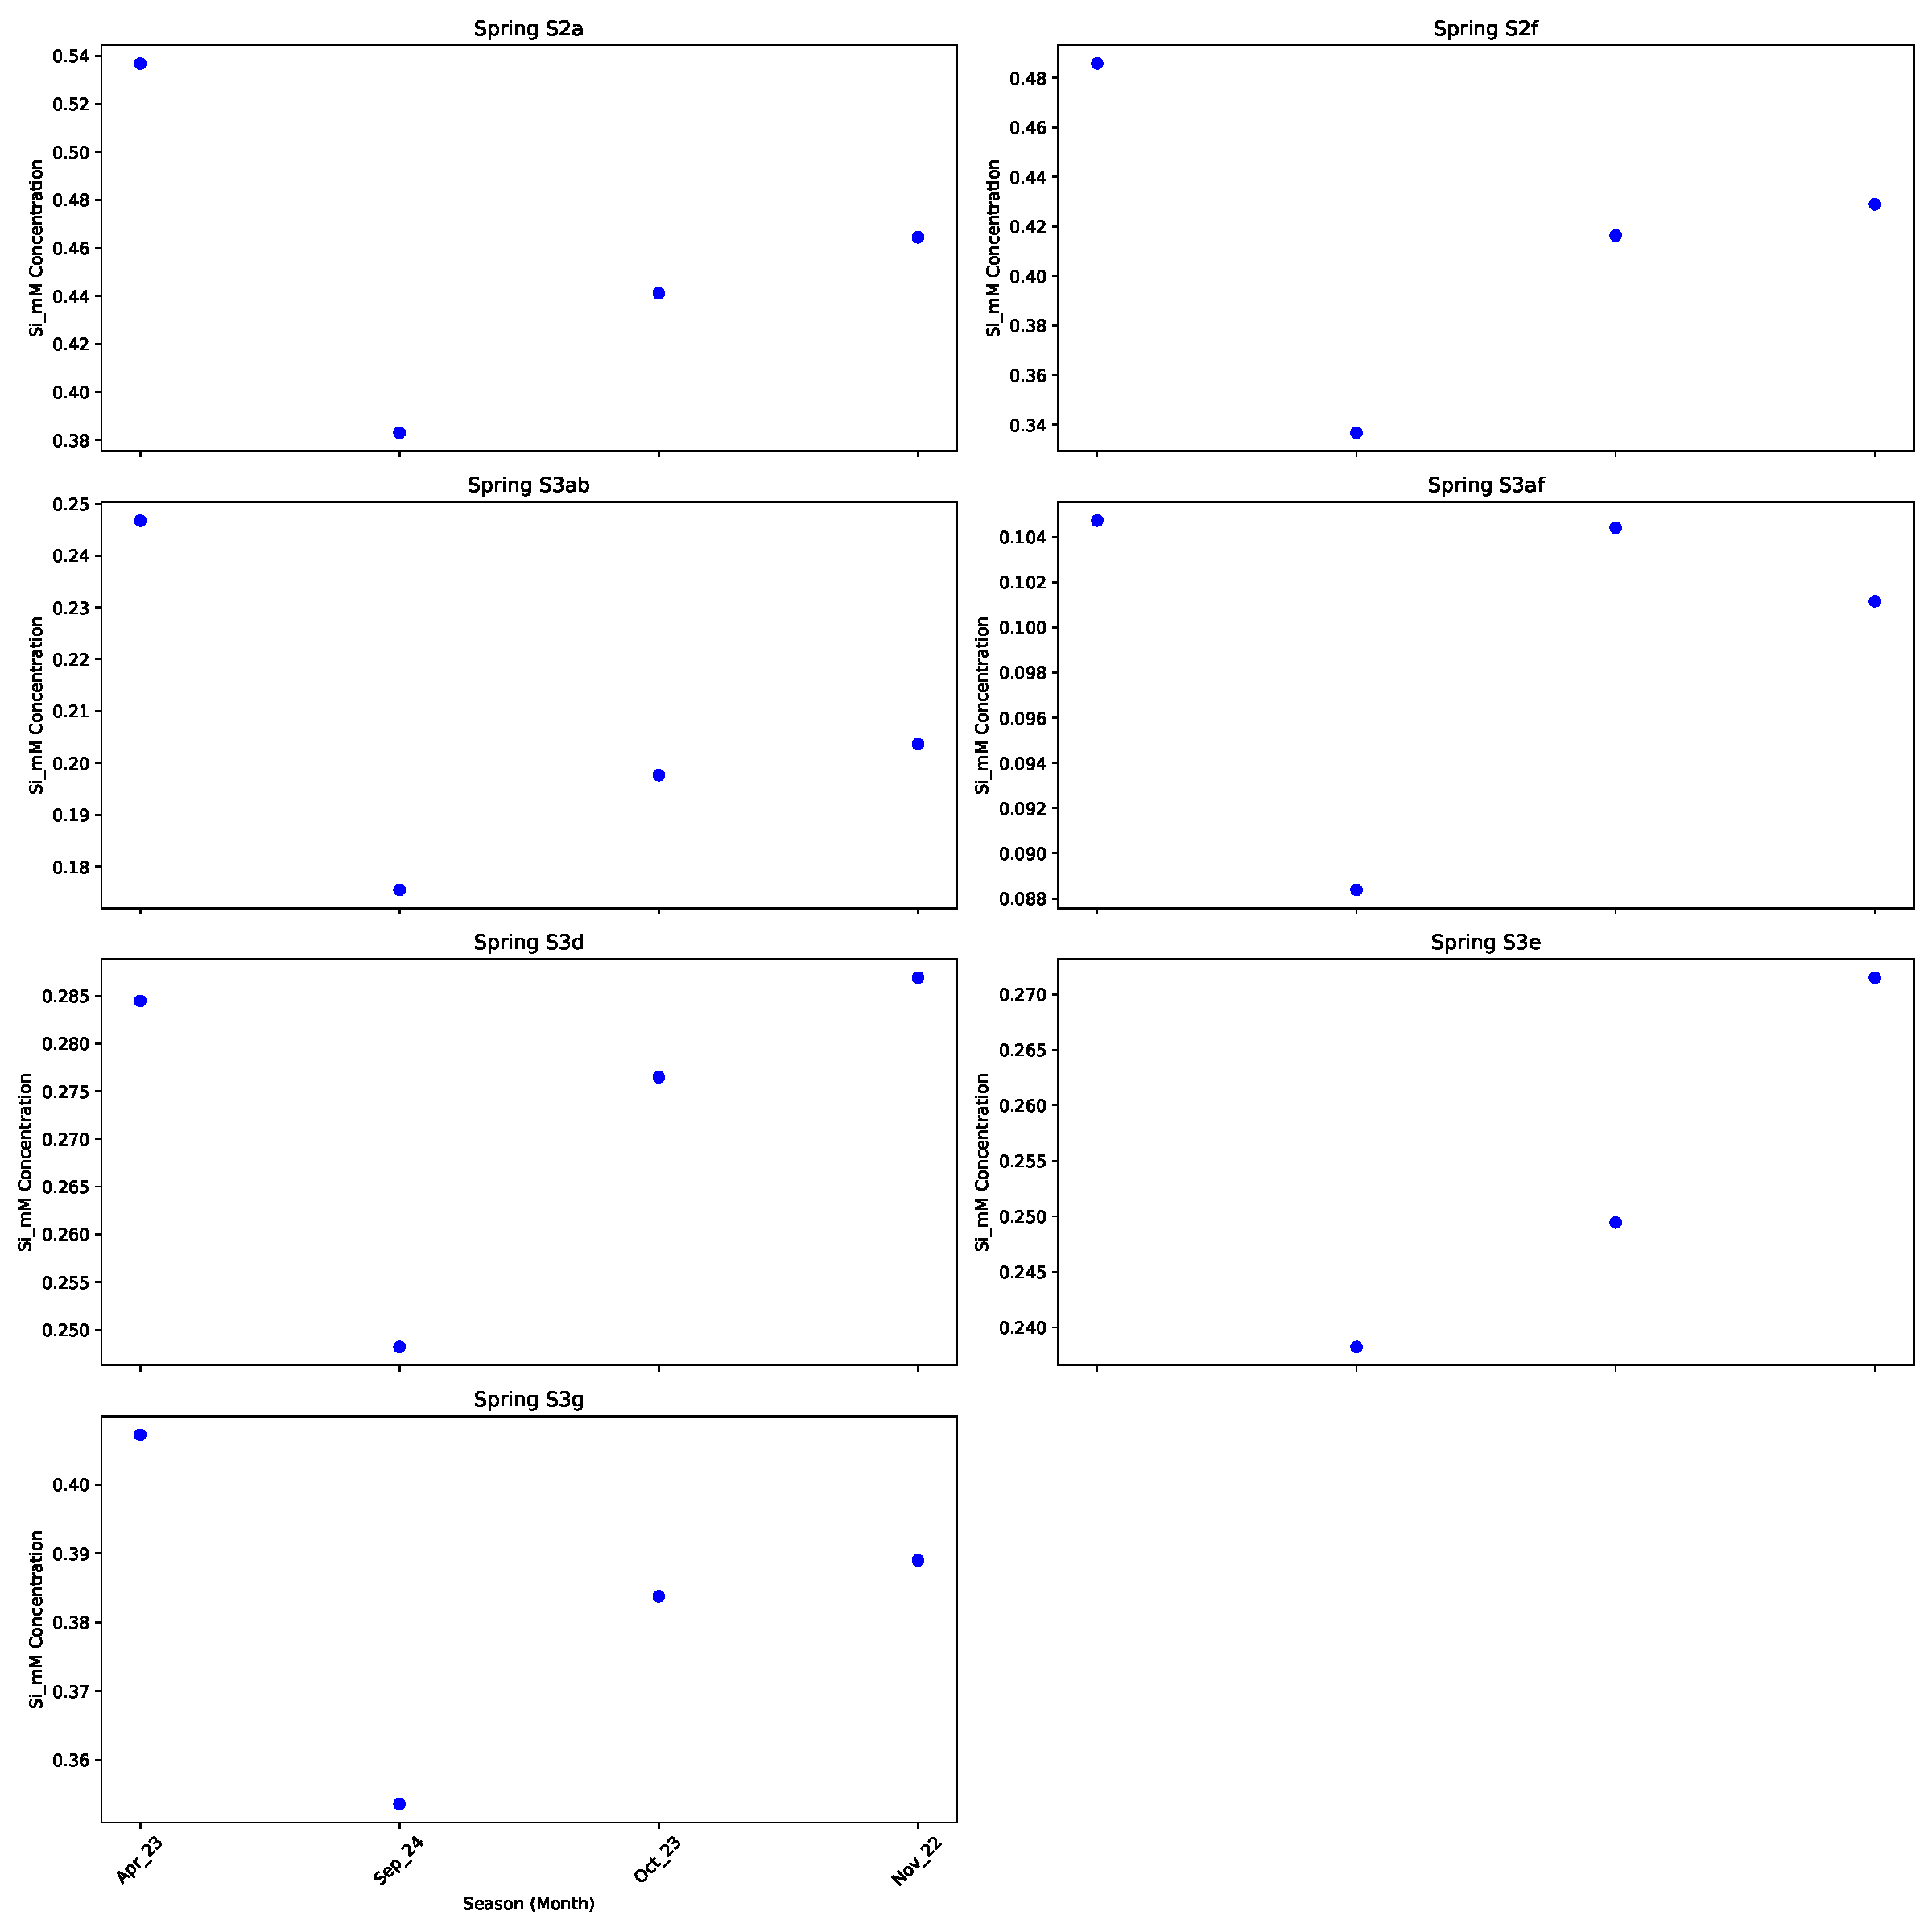
\includegraphics[width=0.8\textwidth]{Si_mM_concentrations_springs.pdf}
    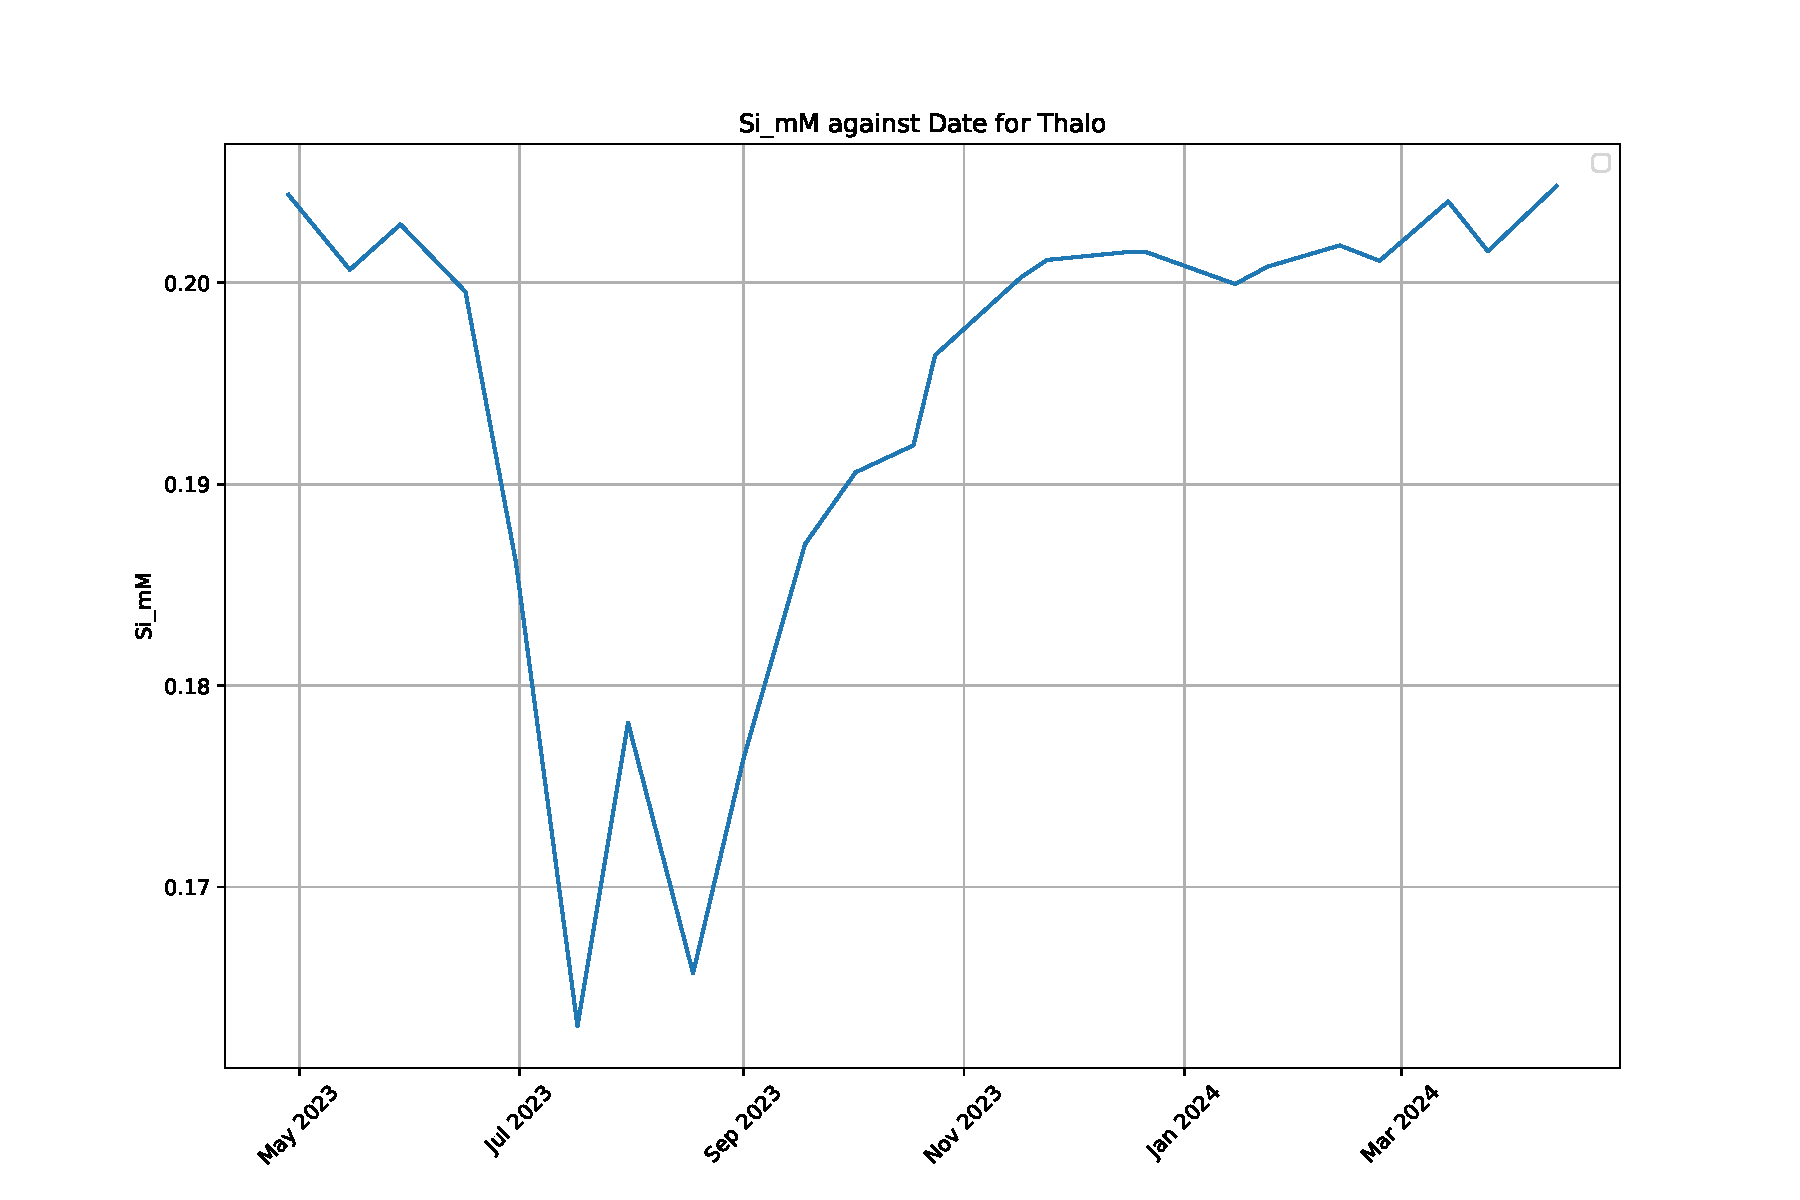
\includegraphics[width=0.8\textwidth]{Si_mM_Thalo_timeseries.pdf}
    \caption{Seasonal changes in spring concentration indicating monsoonal precipitation influence.; Time series of spring concentration changes over time.}
    \label{fig:time_series_changes}
\end{figure}

\FloatBarrier

\bsk

Recorded temperature at the end of the spring flow paths is variable with the season, and is coldest at the end of the monsoon in November. All seasons show a temperature decrease with increasing elevation, suggesting consistent sampling of spring flow paths. 
\textcolor{red}{Spring temperature is close to lapse rate (what ref?)} 


\begin{figure}[h]
    \centering
    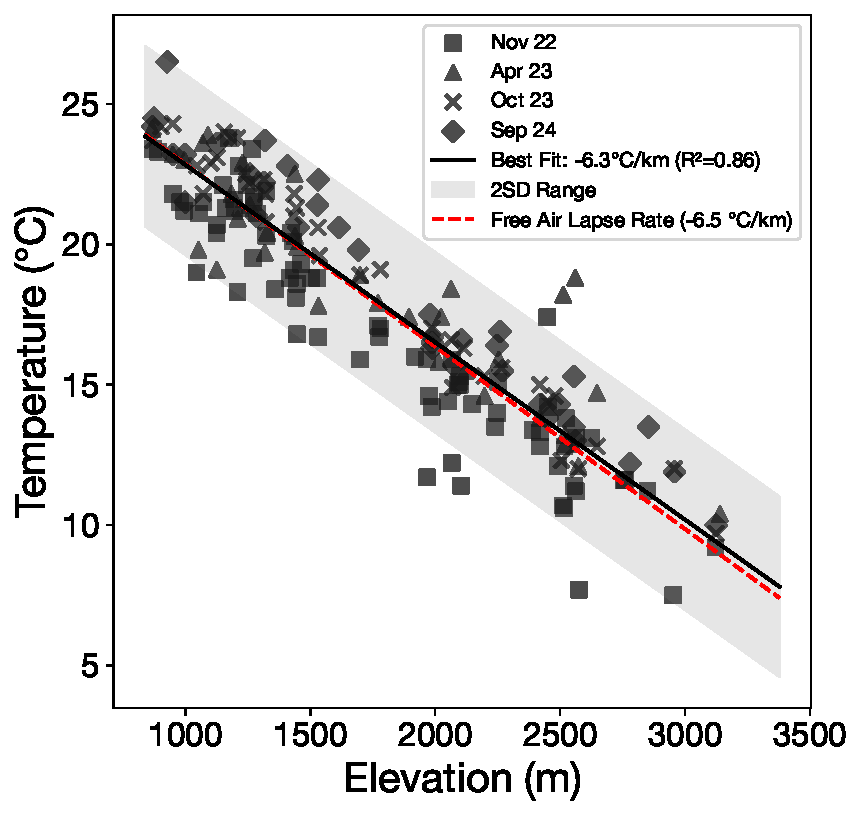
\includegraphics[width=\textwidth]{Temperature_Elevation_Season.pdf}
    \caption{Temperature cahnges}
    \label{fig:seasonal_change2}
\end{figure}

\FloatBarrier

\newpage


\subsection{Spatial concentration changes between the springs}

Broadly, the northernmost three traverses display a linear trend of concentration and alkalinity with elevation \textcolor{red}{Alkalinity slightly different...} . The southernmost two traverses display a distinct jump in concentration. This could suggest that the springs sampled tap into different lithologies, but this could also be due to longer flow paths and a closer approach to equilibrium. The possible controls on these variations, namely temperature, flow path length, lithology, dissolution rates, and evapotratnspiration cannot easily be distinguished.

\begin{figure}[h]
    \centering
    \begin{tabular}{c}
        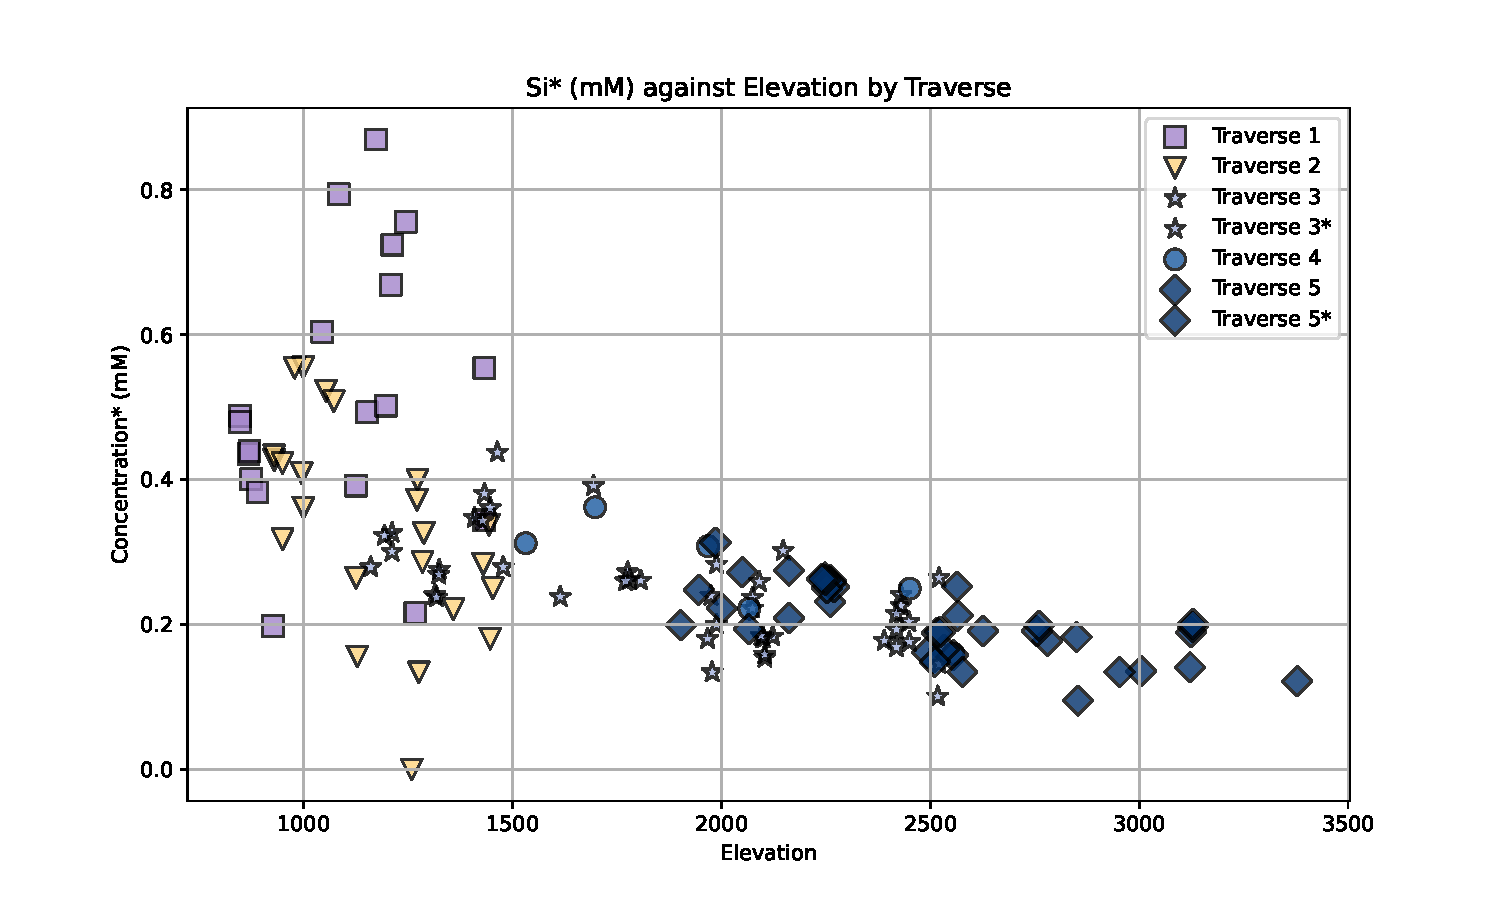
\includegraphics[width=0.8\textwidth]{Si_mM_EC_Elevation.pdf} \\
        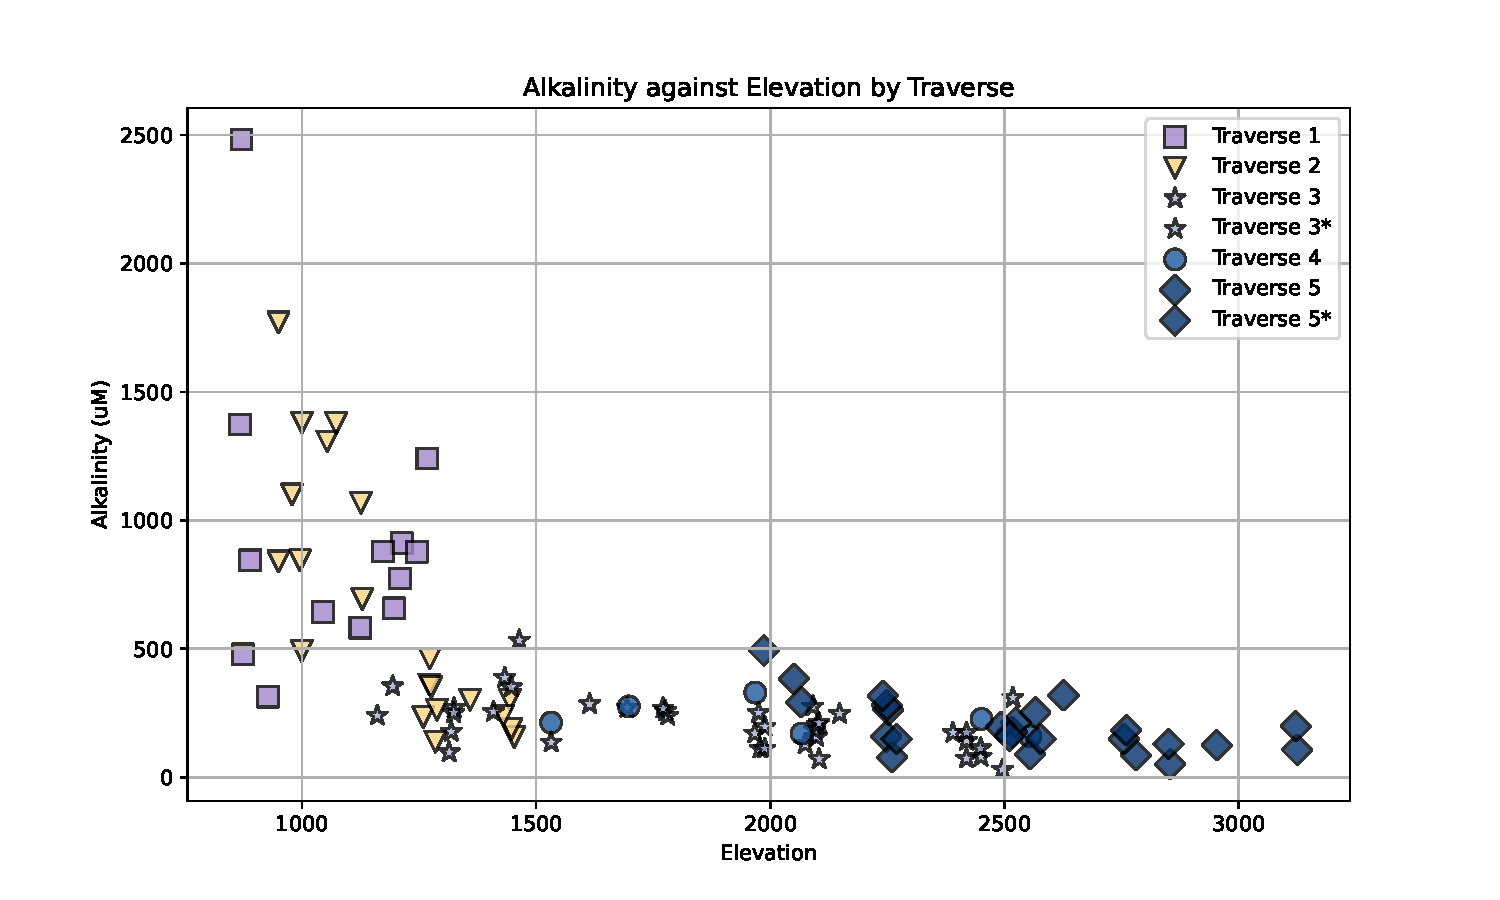
\includegraphics[width=0.8\textwidth]{Alkalinity_Elevation.pdf} \\
    \end{tabular}
    \caption{How Alkalinity and Si changes with elevation}
    \label{fig:spatial_changes_spring2}
\end{figure}

\FloatBarrier

% \begin{figure}[h]
%     \centering
%     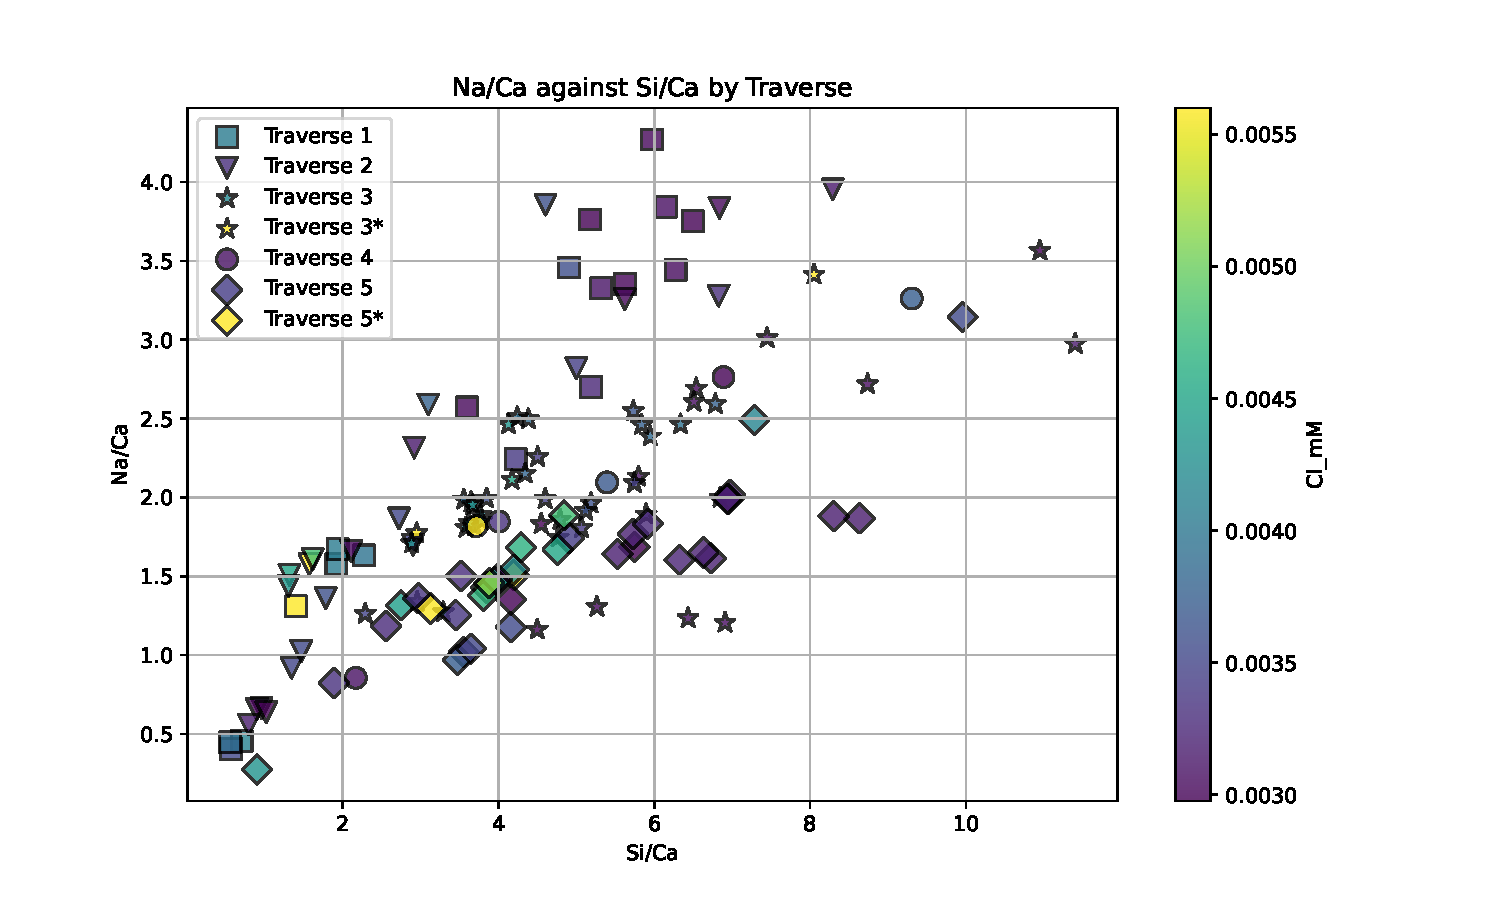
\includegraphics[width=\textwidth]{SiCaNaCa.pdf}
%     \caption{Si/Ca against Na/Ca. Clear differences between traverses.}
%     \label{fig:spatial_changes_spring3}
% \end{figure}



% \begin{figure}[h]
%     \centering
%     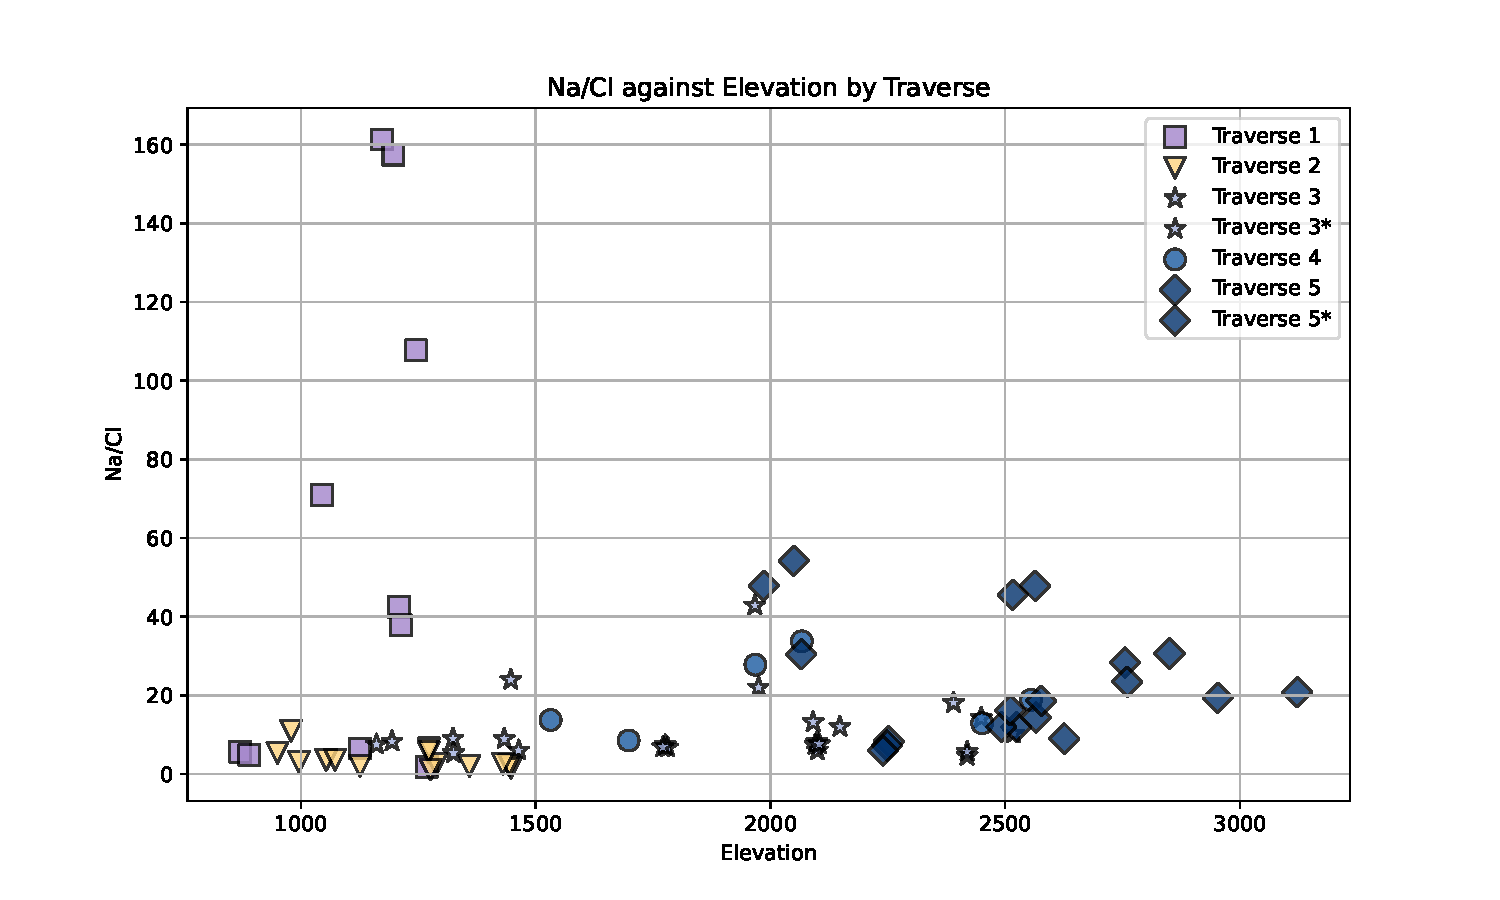
\includegraphics[width=\textwidth]{NaClEl.pdf}
%     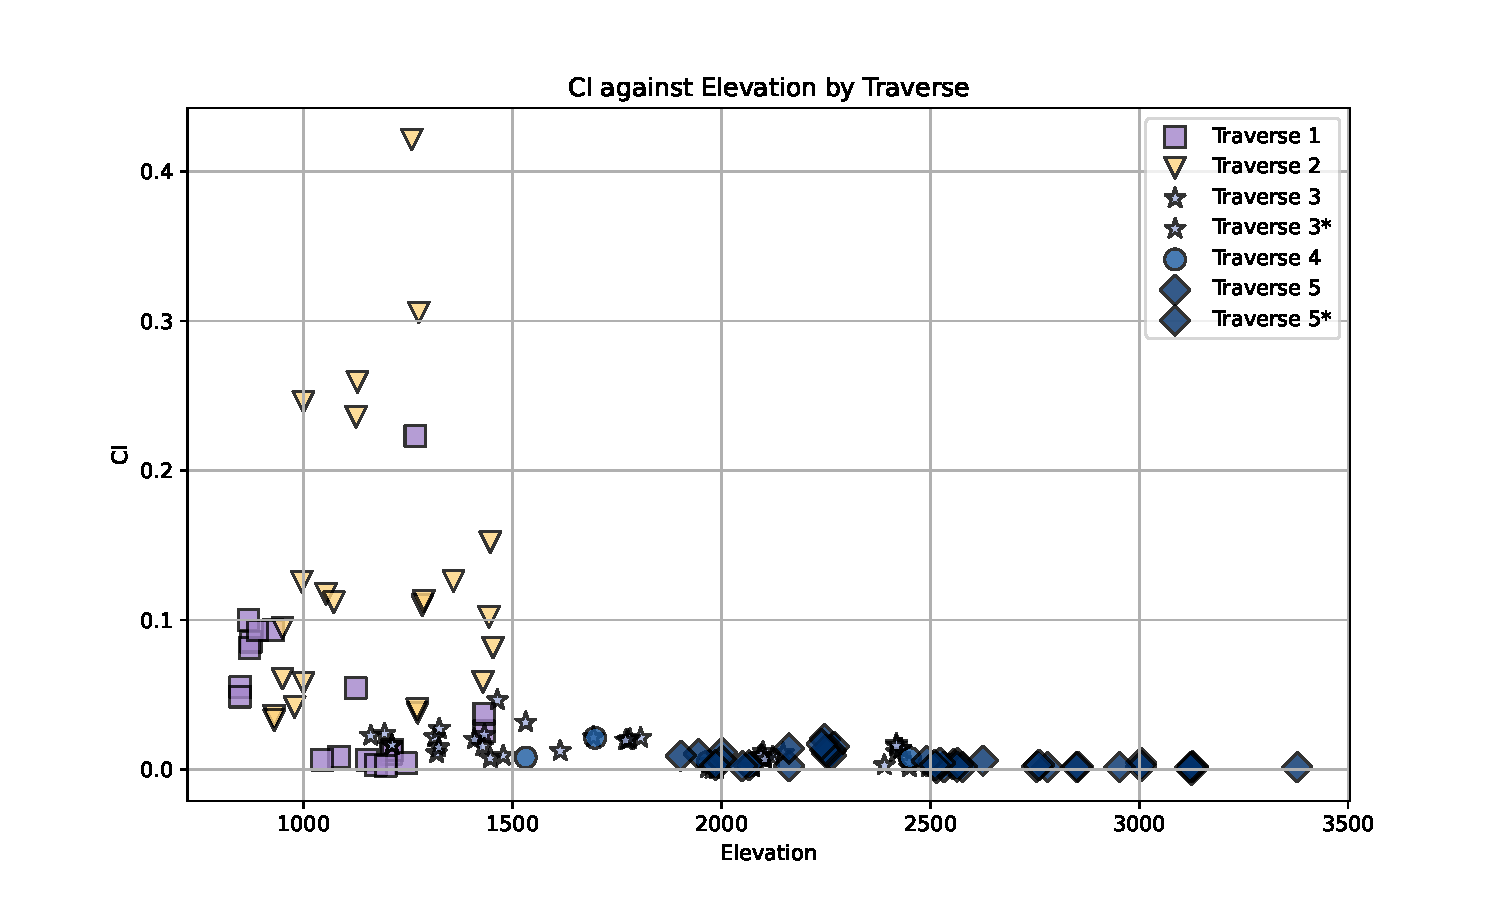
\includegraphics[width=\textwidth]{ClEl.pdf}
%     \caption{NaCl against elevation coloured by traverse -  super low Cl; Cl against elevation coloured by traverse - Potential evaporite influence on traverse 2 water chemistry}
%     \label{fig:spatial_changes_spring5}
% \end{figure}

% \FloatBarrier

\newpage


\subsection{Sr isotope against 1/Sr data \textcolor{red}{Change title} }
\textcolor{red}{make this whole subsection simpler} 
Radiogenic strontium isotope analyses of springs similarly show a wide variation between different traverses. Due to the unique source-tracking nature of strontium isotopes this is potentially explained with varying lithology along the ridge. These variations are however consistent with the range of Higher Himalayan Crystalline Series (HHCS) rocks found in the region (Tipper et al., 2006), so it is unlikely that the source of the Sr isotopes is from the Lesser Himalayan Series (LHS) rocks - the MCT is quite a bit more south than this \textcolor{red}{Make this sentence simpler} .

\bsk

Sr isotopes derived from the most recent rain analyses are of the order of 0.70904 to 0.70925 at the lowest. Seawater is of the order of 0.70917. Within error, therefore, the lowest rain values reflect seawater strontium isotope values, indicating little contamination from dust or particles. The non-contaminated samples are indeed found at the higher elevations, and they show low chloride concentrations consistent with rain. \textcolor{red}{Need a table with errors} 

\bsk

Compared to the springs on a 87Sr/86Sr against 1Sr plot (Figure 5D eg), there is no significant spring mixing line towards the rain. This suggests that the spring water undergoes significant chemical weathering compared to the initial input, suggesting long flow paths and/or long residence times.


\begin{figure}[p]
    \centering
    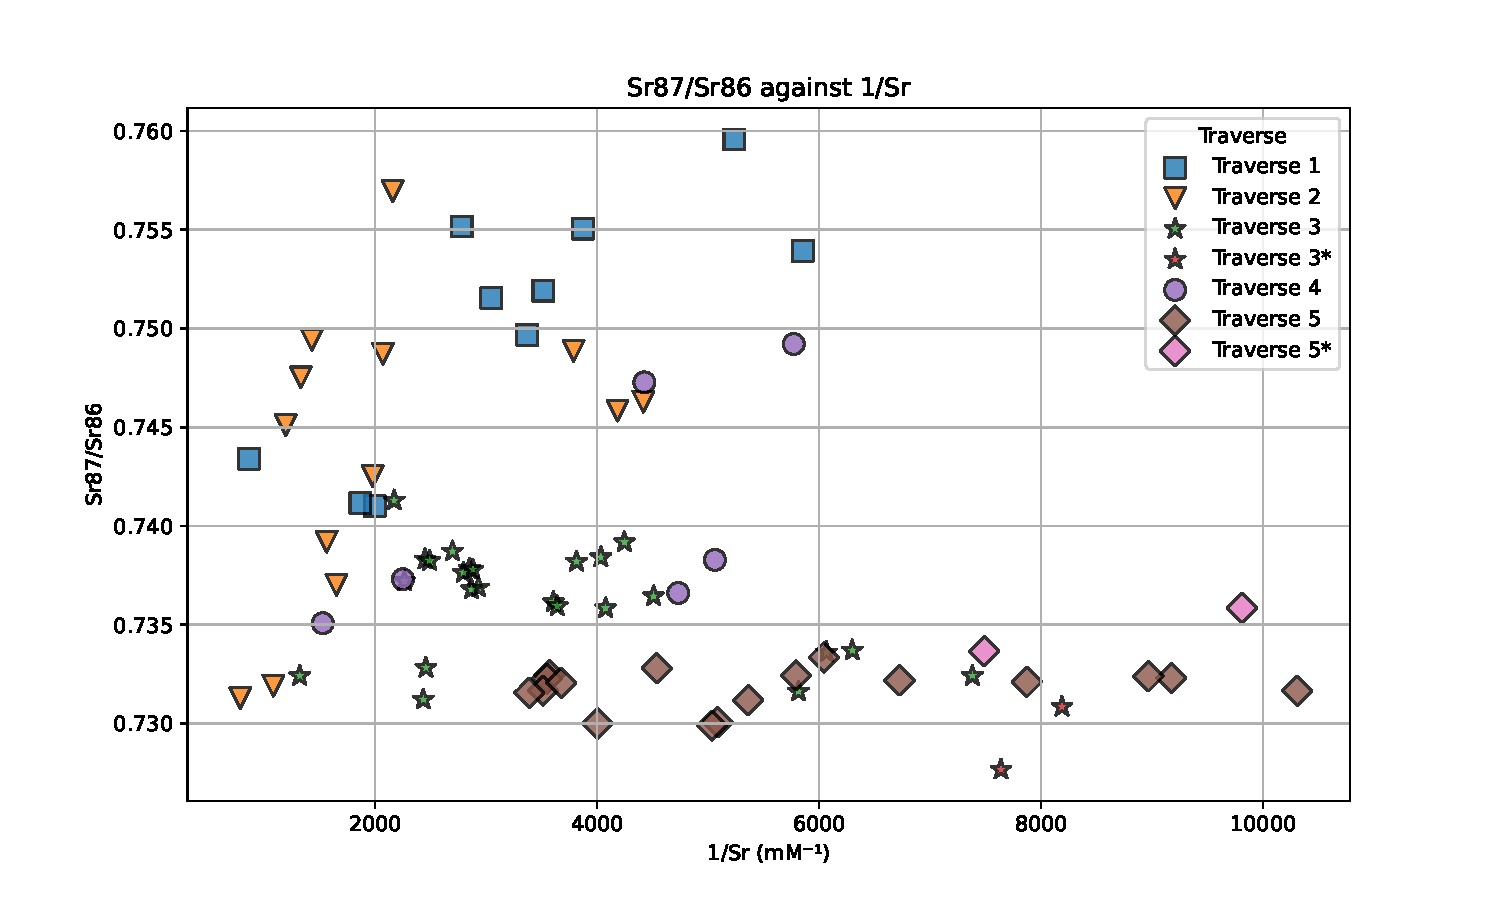
\includegraphics[width=\textwidth]{Sr87_Sr86_1_Sr.pdf}
    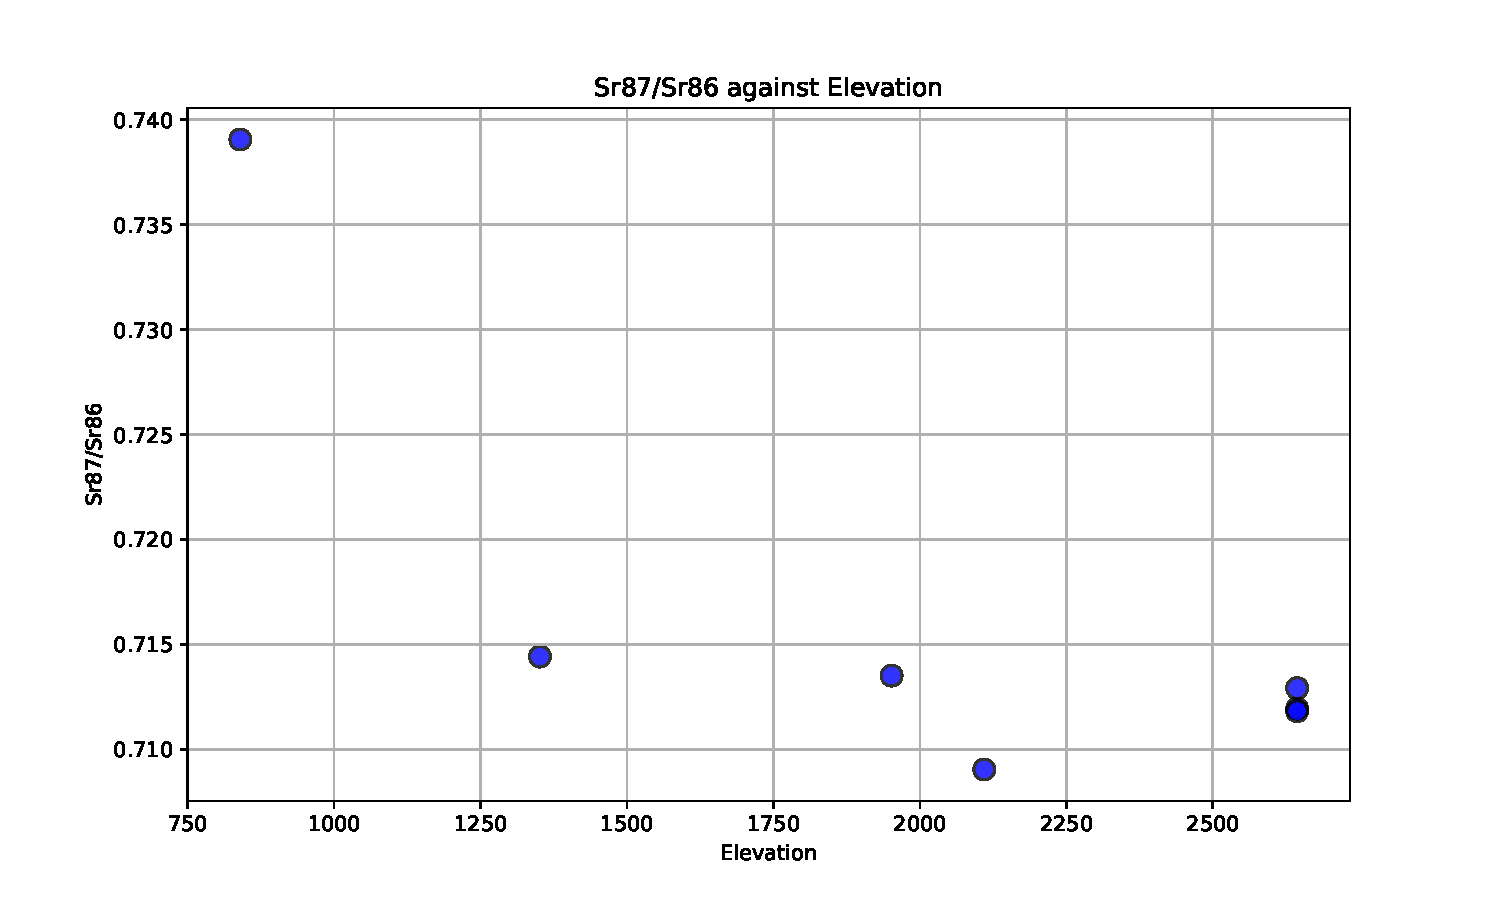
\includegraphics[width=\textwidth]{Sr87_Sr86_Elevation.pdf}
    \caption{Strontium isotope differences display difference in lithology tapped in. Cite Quade and Tipper papers; Rain analysed for Sr isotopes and Cl. Something about contamination lower down; How samples of Traverse 3 compare to the rain samples}
    \label{fig:discussion3}
\end{figure}

\begin{figure}[p]\ContinuedFloat
    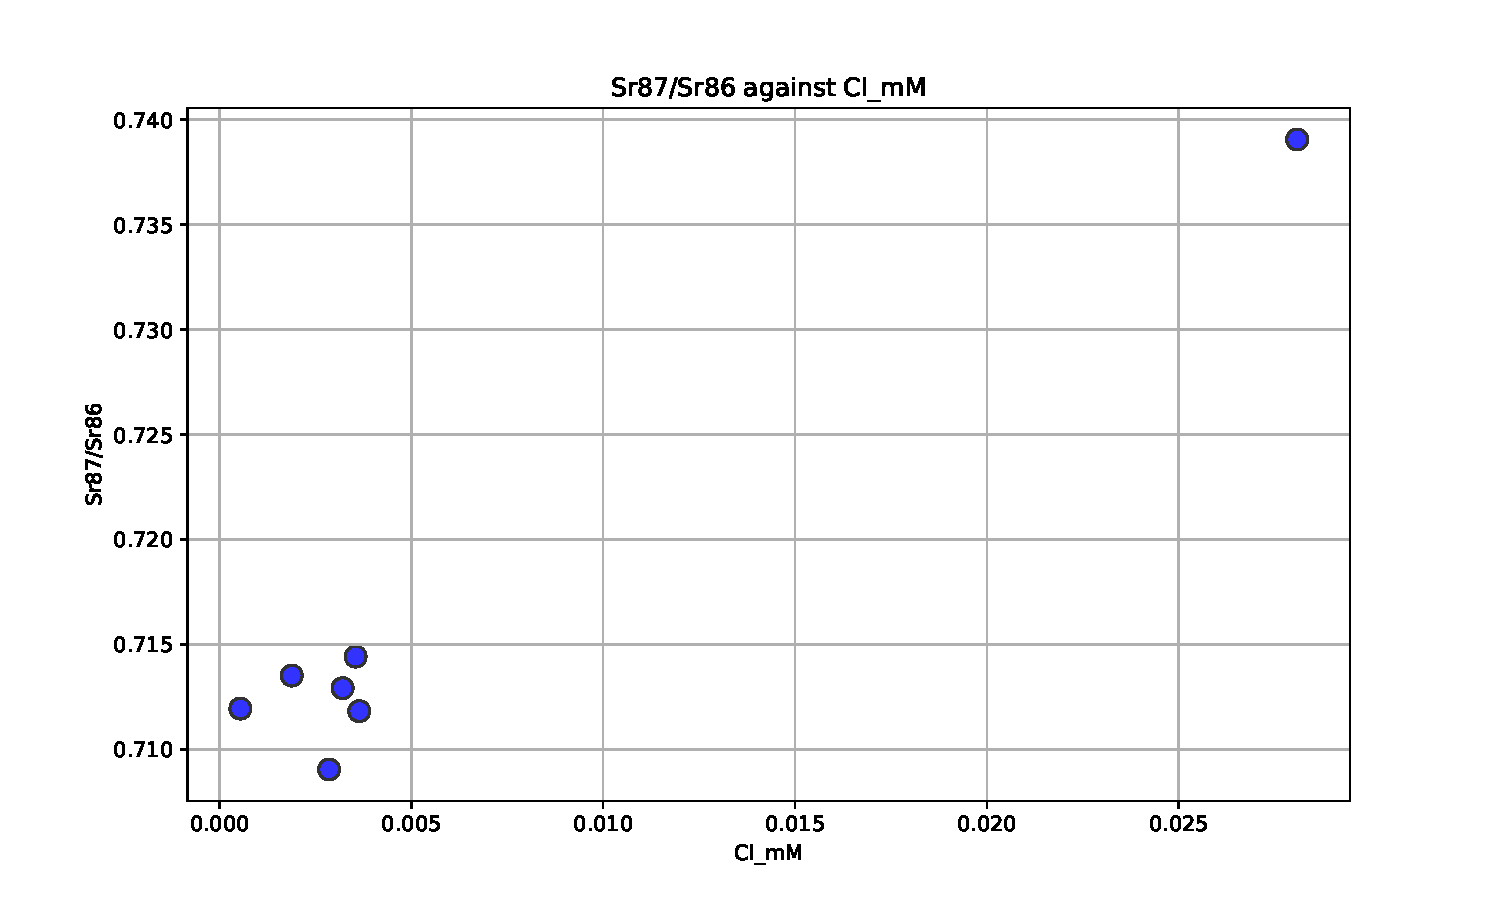
\includegraphics[width=\textwidth]{Sr87_Sr86_Cl.pdf}
    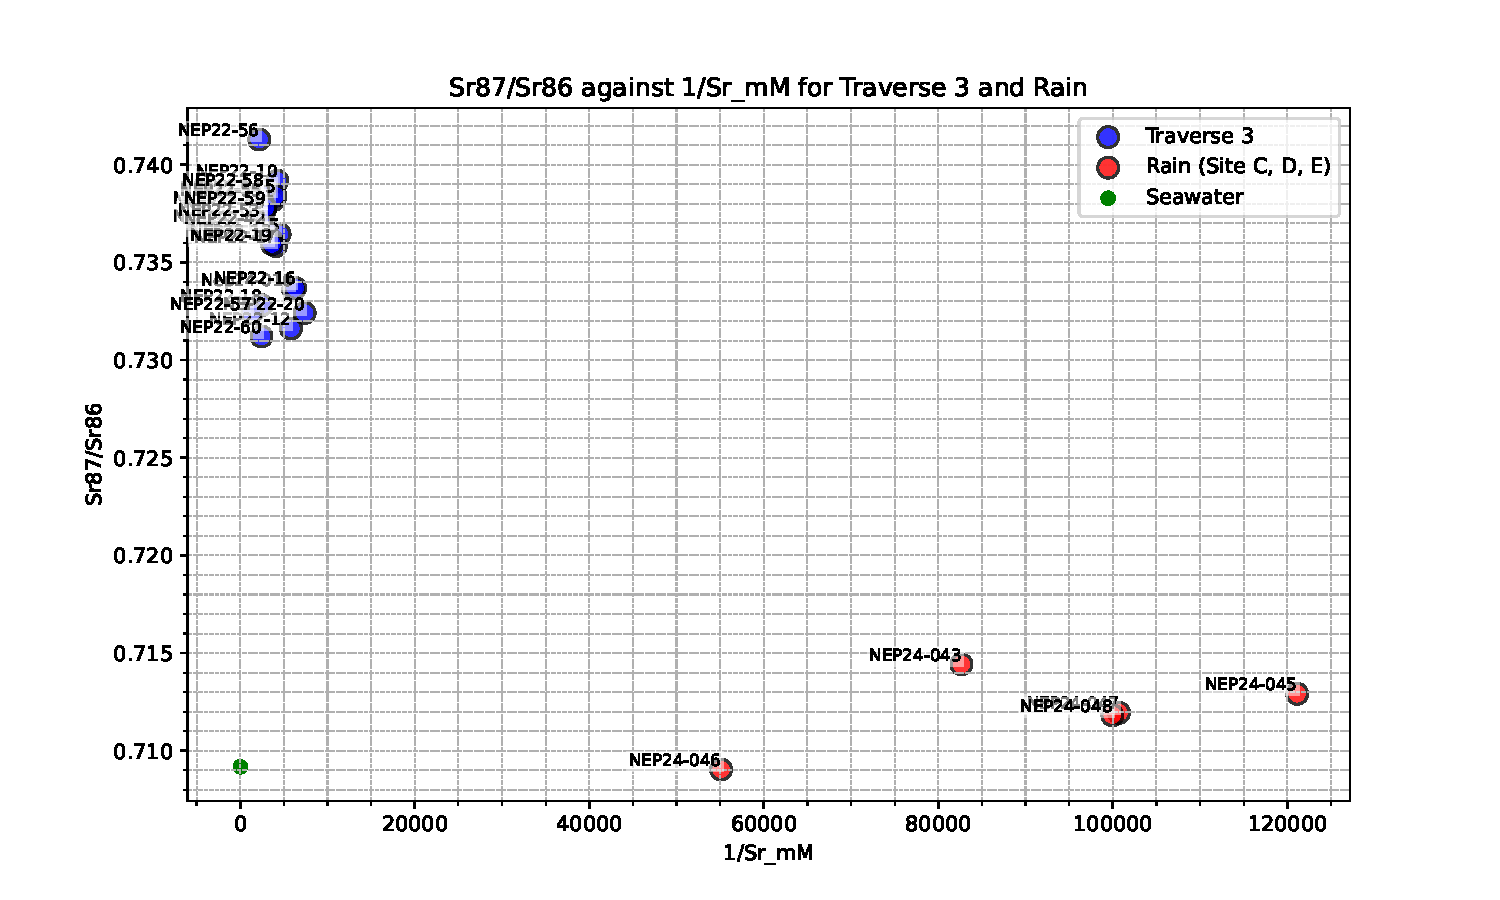
\includegraphics[width=\textwidth]{Sr87_Sr86_1Sr_Rain.pdf}
    \caption[]{(Continued)}
\end{figure}

\FloatBarrier

% \begin{figure}[h]
%     \centering
%     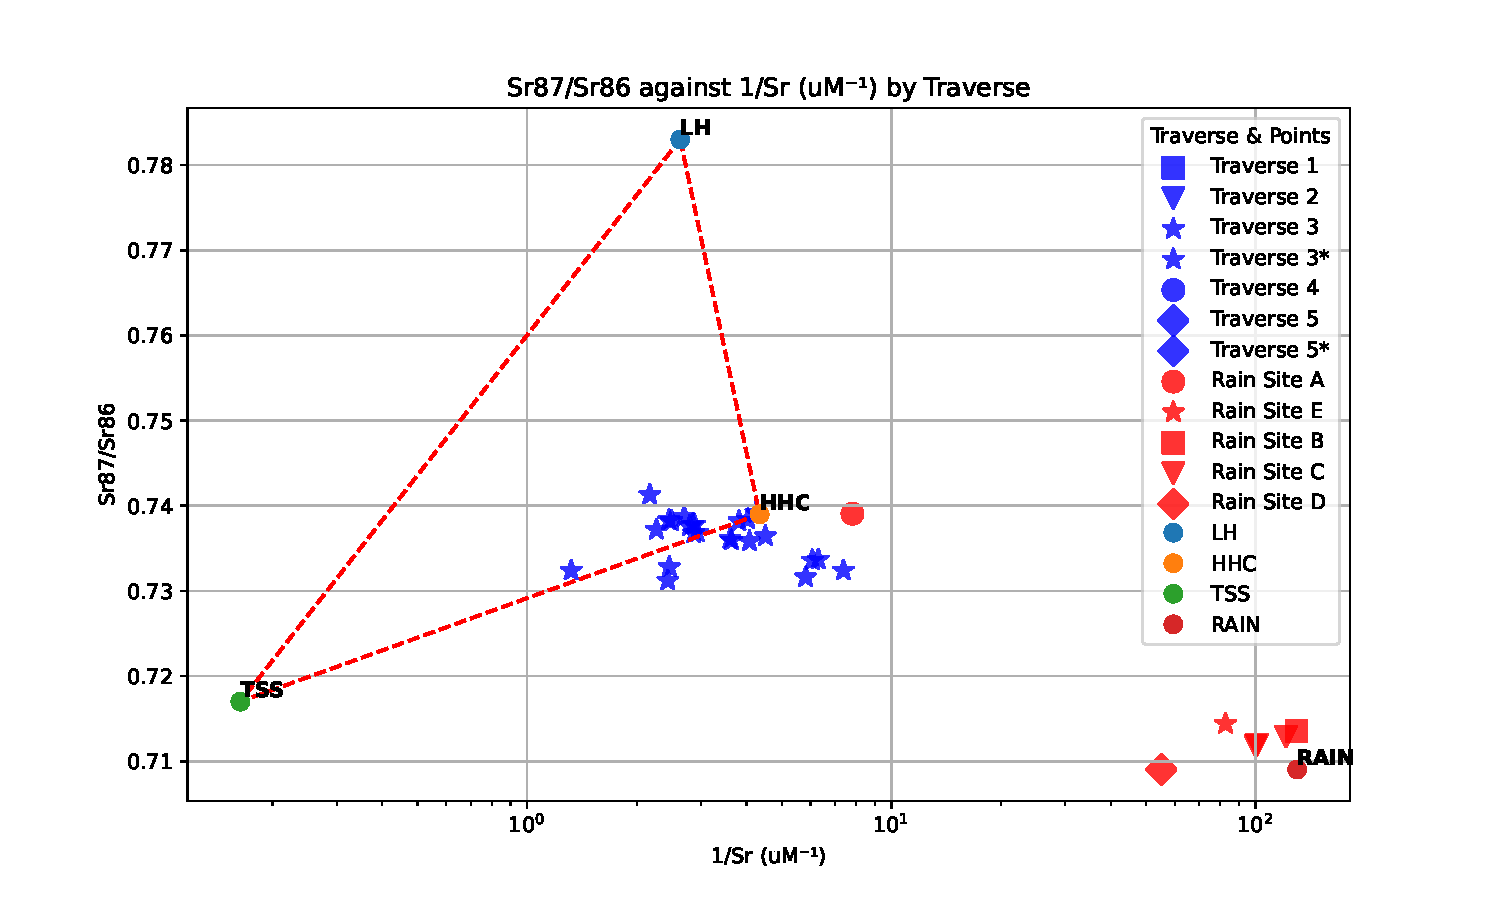
\includegraphics[width=\textwidth]{Sr87_Sr86_1Sr_Traverse_Triangle.pdf}
%     \caption{Recreating the Lanord plot etc. Need to choose better endmembers}
%     \label{fig:discussion4}
% \end{figure}

% Also include 87Sr/86Sr weathering according to that mass balance thing... if that helps

\newpage

\subsection{Traverse 3 is the best sampled and least influenced - \textcolor{red}{Need a better title}}

It is difficult to explain the inter-traverse variation in concentration and isotopic composition. As a result, for the remainder of this study's analysis, only Traverse 3 out of the five will be chosen as a case study representing the catchment. Whilst it is also possible that all traverses' flow paths are connected one to the other \textcolor{red}{something about just traverse 3}. This is because, for traverse 3, there is little evidence to suggest lithology is not constant. For one, geological maps suggest lithology does not vary across E-W, which is the profile all traverses follow. Secondly as is evident from the Na/Si against itself plot, Na/Si plots almost exactly on the 1:1 line for every season where the same spring was sampled in Traverse 3. The fact that this ratio increases with decreasing elevation suggests more and more Si is reprecipitated, while Na is only involved in dissolution. The narrow range and tight scatter suggests little lithological change and consistently sampled flow paths over time. This is even more apparent when plotting against elevation for different seasons.

\begin{figure}[p]
    \centering
    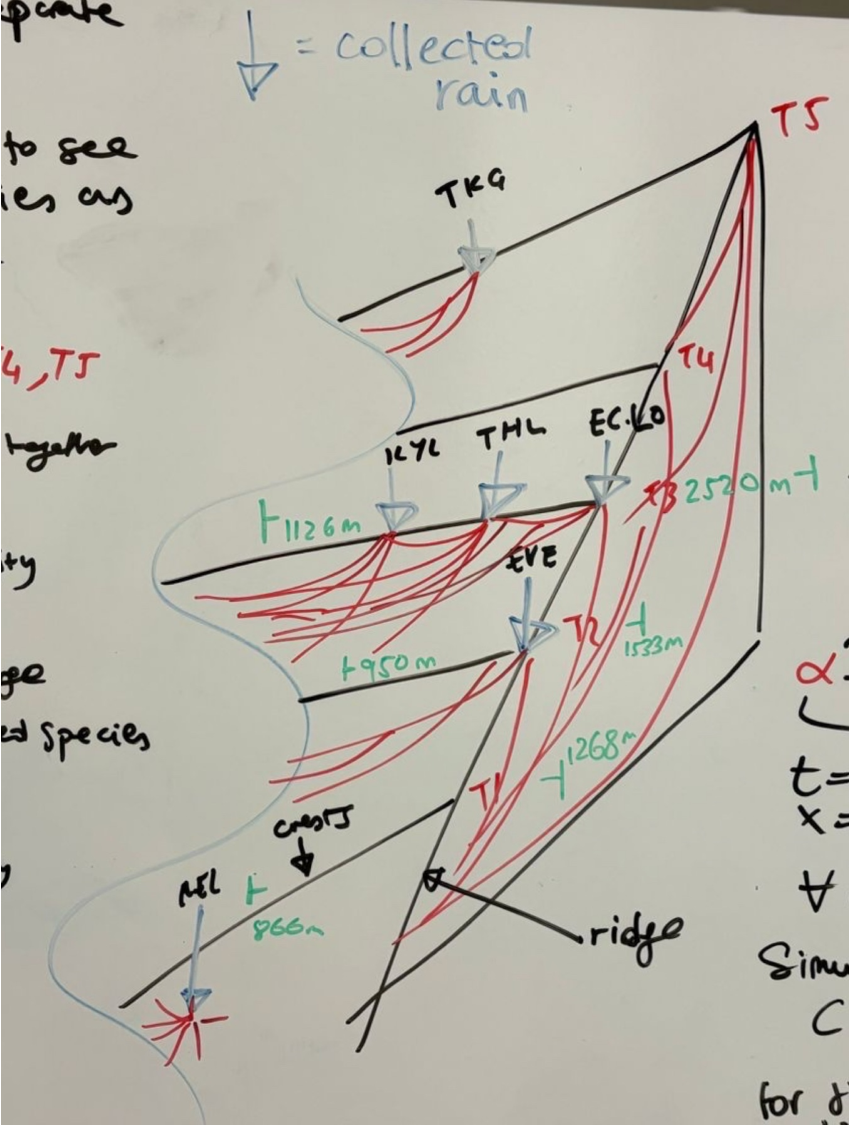
\includegraphics[width=0.5\textwidth]{ExampleFlow.pdf}
    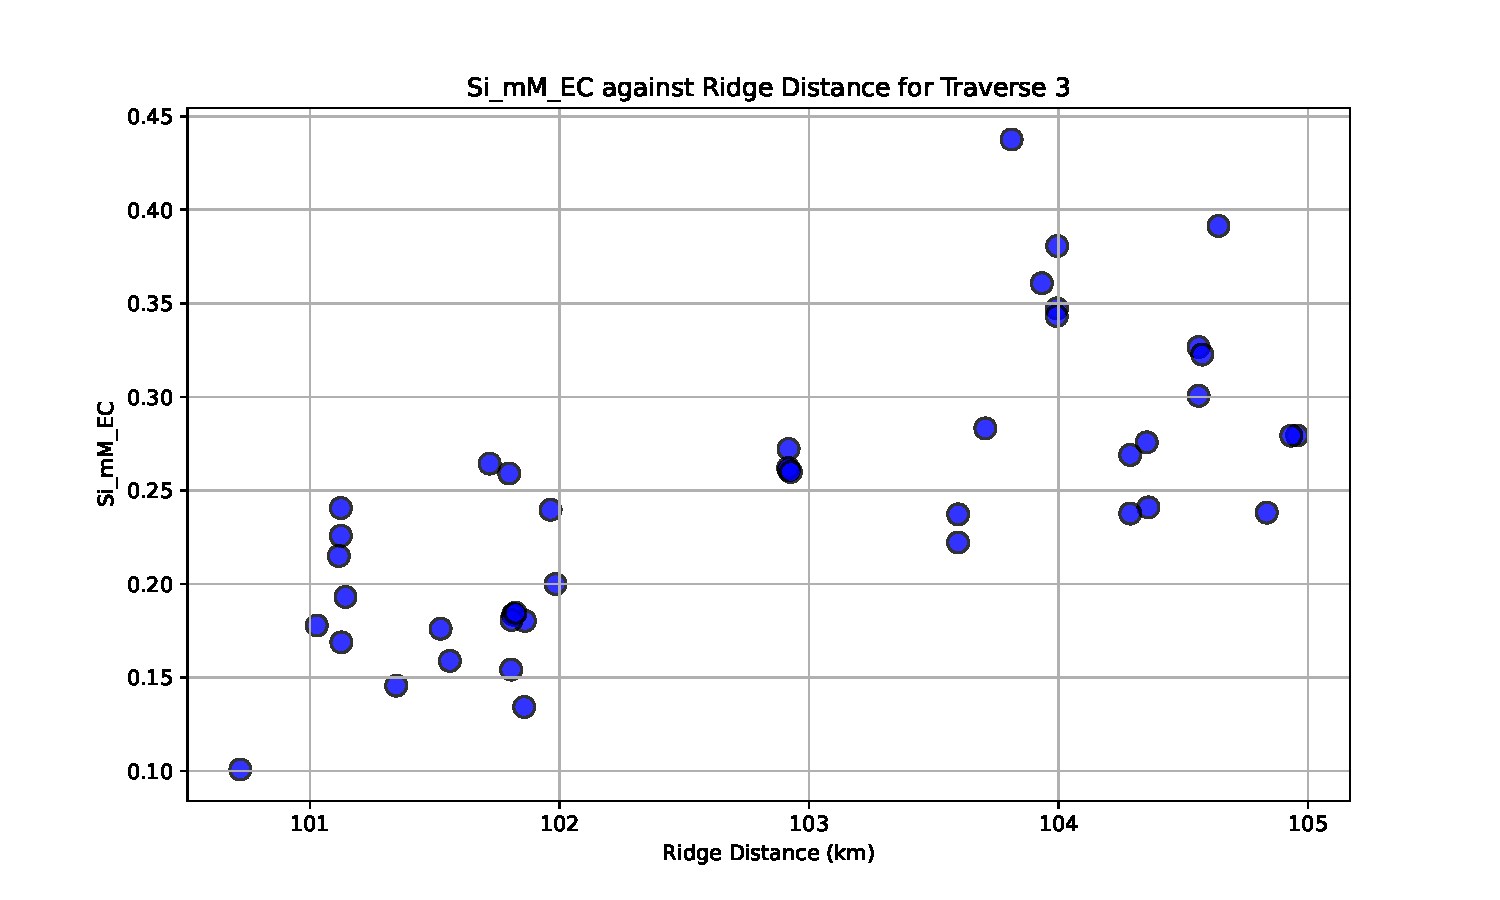
\includegraphics[width=\textwidth]{Si_mM_EC_Ridge_Distance.pdf}
    \caption{How Si varies for Traverse 3, showing a wide variety of samples; Na/Si for Traverse 3 is pretty neat. Consistently sampled flow paths.}
    \label{fig:spatial_changes_spring8}
\end{figure}

\begin{figure}[p]\ContinuedFloat
    \centering
    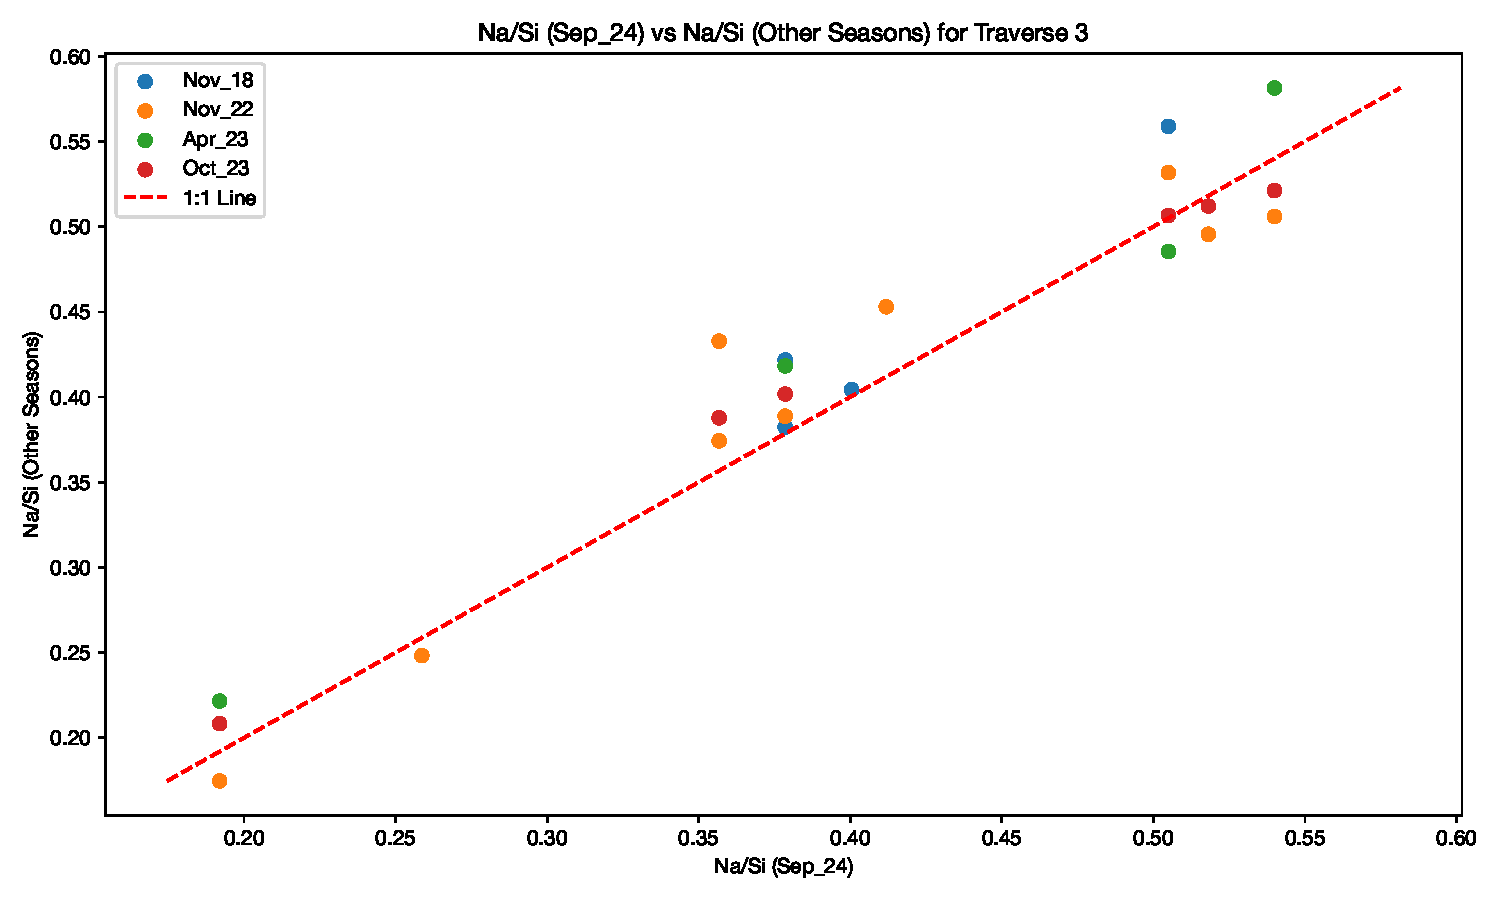
\includegraphics[width=\textwidth]{Na_Si_Trav3.pdf}
    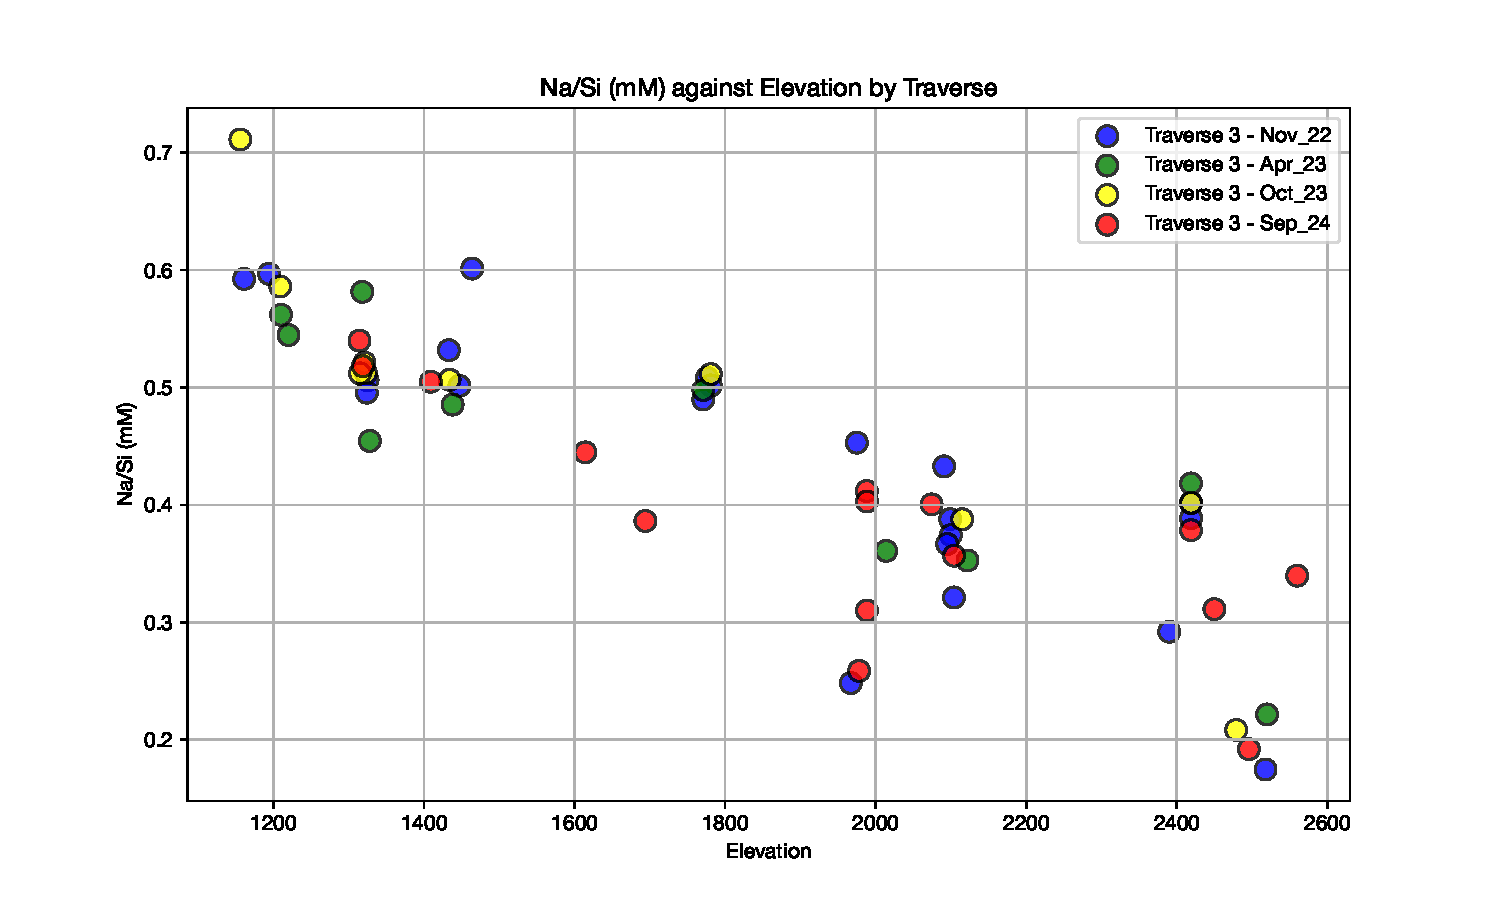
\includegraphics[width=\textwidth]{Na_Si_Elevation.pdf}
    \caption[]{(Continued)}
\end{figure}

\FloatBarrier


% \begin{figure}[h]
%     \centering
%     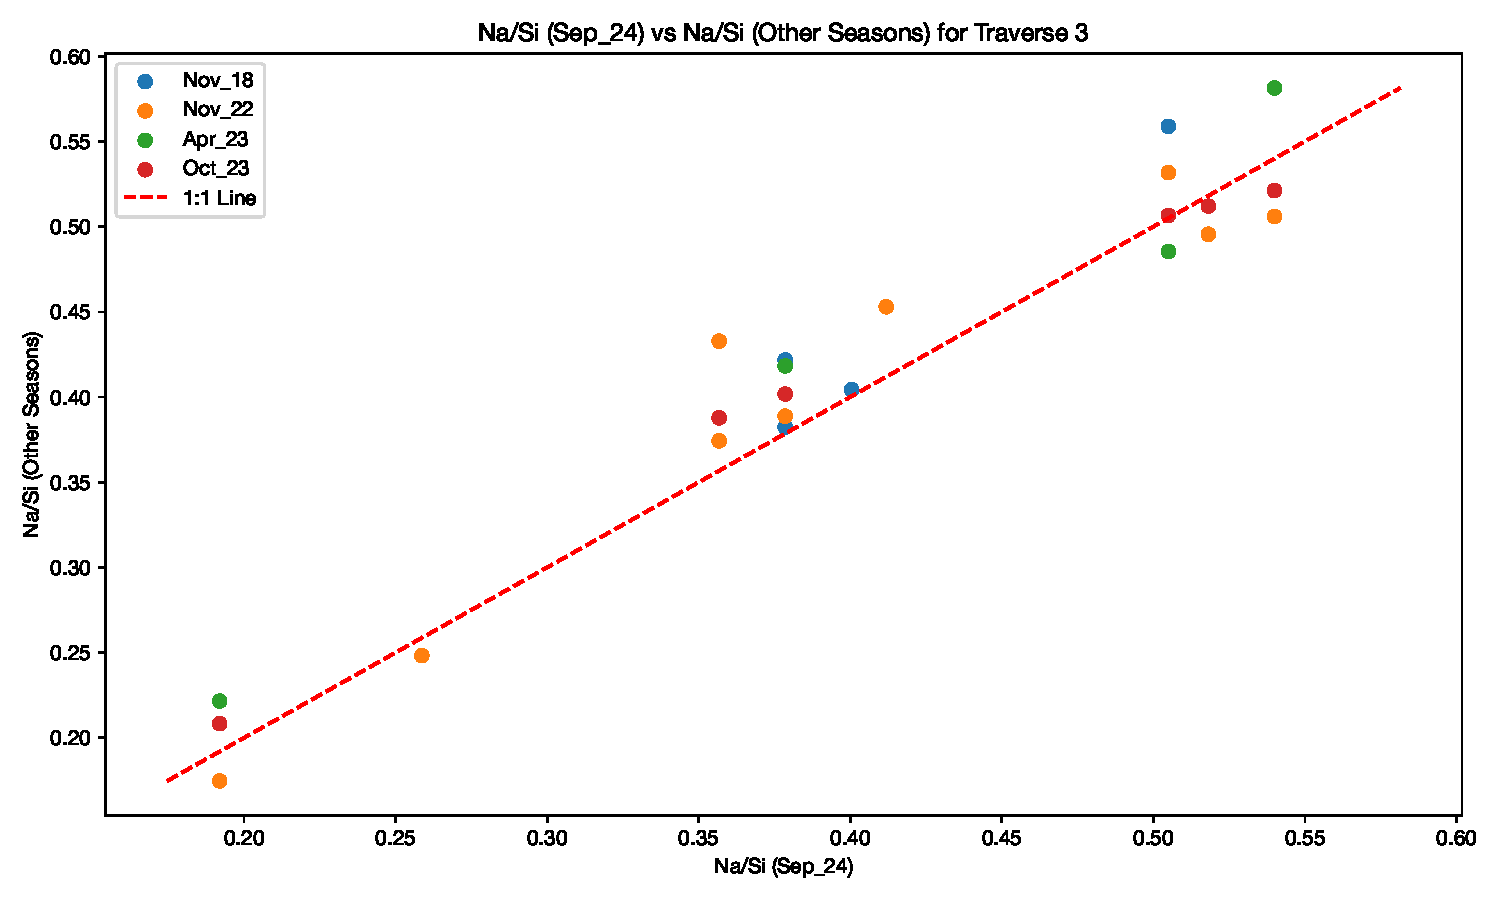
\includegraphics[width=\textwidth]{Na_Si_Trav3.pdf}
%     \caption{Na/Si for Traverse 3 is pretty neat}
%     \label{fig:spatial_changes_spring9}
% \end{figure}

% \FloatBarrier



